\chapter{Systembeskrivelse} \label{ch:Systembeskrivelse}
Systemet består samlet af en PC, en Xbox-360 controller og en legetøjsbil, som styres med Xbox-360 controlleren fra PC'en. Legetøjsbilen styres via et netværk som kræver at både PC og bil er logget på samme netværk. Bilen tilkobles en trådløs forbindelse hvorimod PC sagtens kan tilgå netværket via kabel. Bilen er udstyret med et antikollisions system som i resten af rapporten er forkortet til AKS. AKS systemet overtager styringen fra brugeren når bilen styres imod en forhindring, således bilen selv kan manøvrere udenom forhindringen. For at styre bilen fra PC'en med Xbox-360 controlleren skal der installeres en GUI hvori der også modtages video-stream fra et kamera påmonteret bilen. Endvidere modtages der data fra bilen således brugeren kan se den nuværende hastighed, acceleration og afstand til forhindring. Det er også muligt for brugeren af specificere en maksimal hastighed som bilen kan opnå. Se Figur \ref{fig:rigbillede} for samlet system. En skitse af GUI'en er vist i figur \ref{fig:main_menu}.
\begin{figure}[H]
\centering
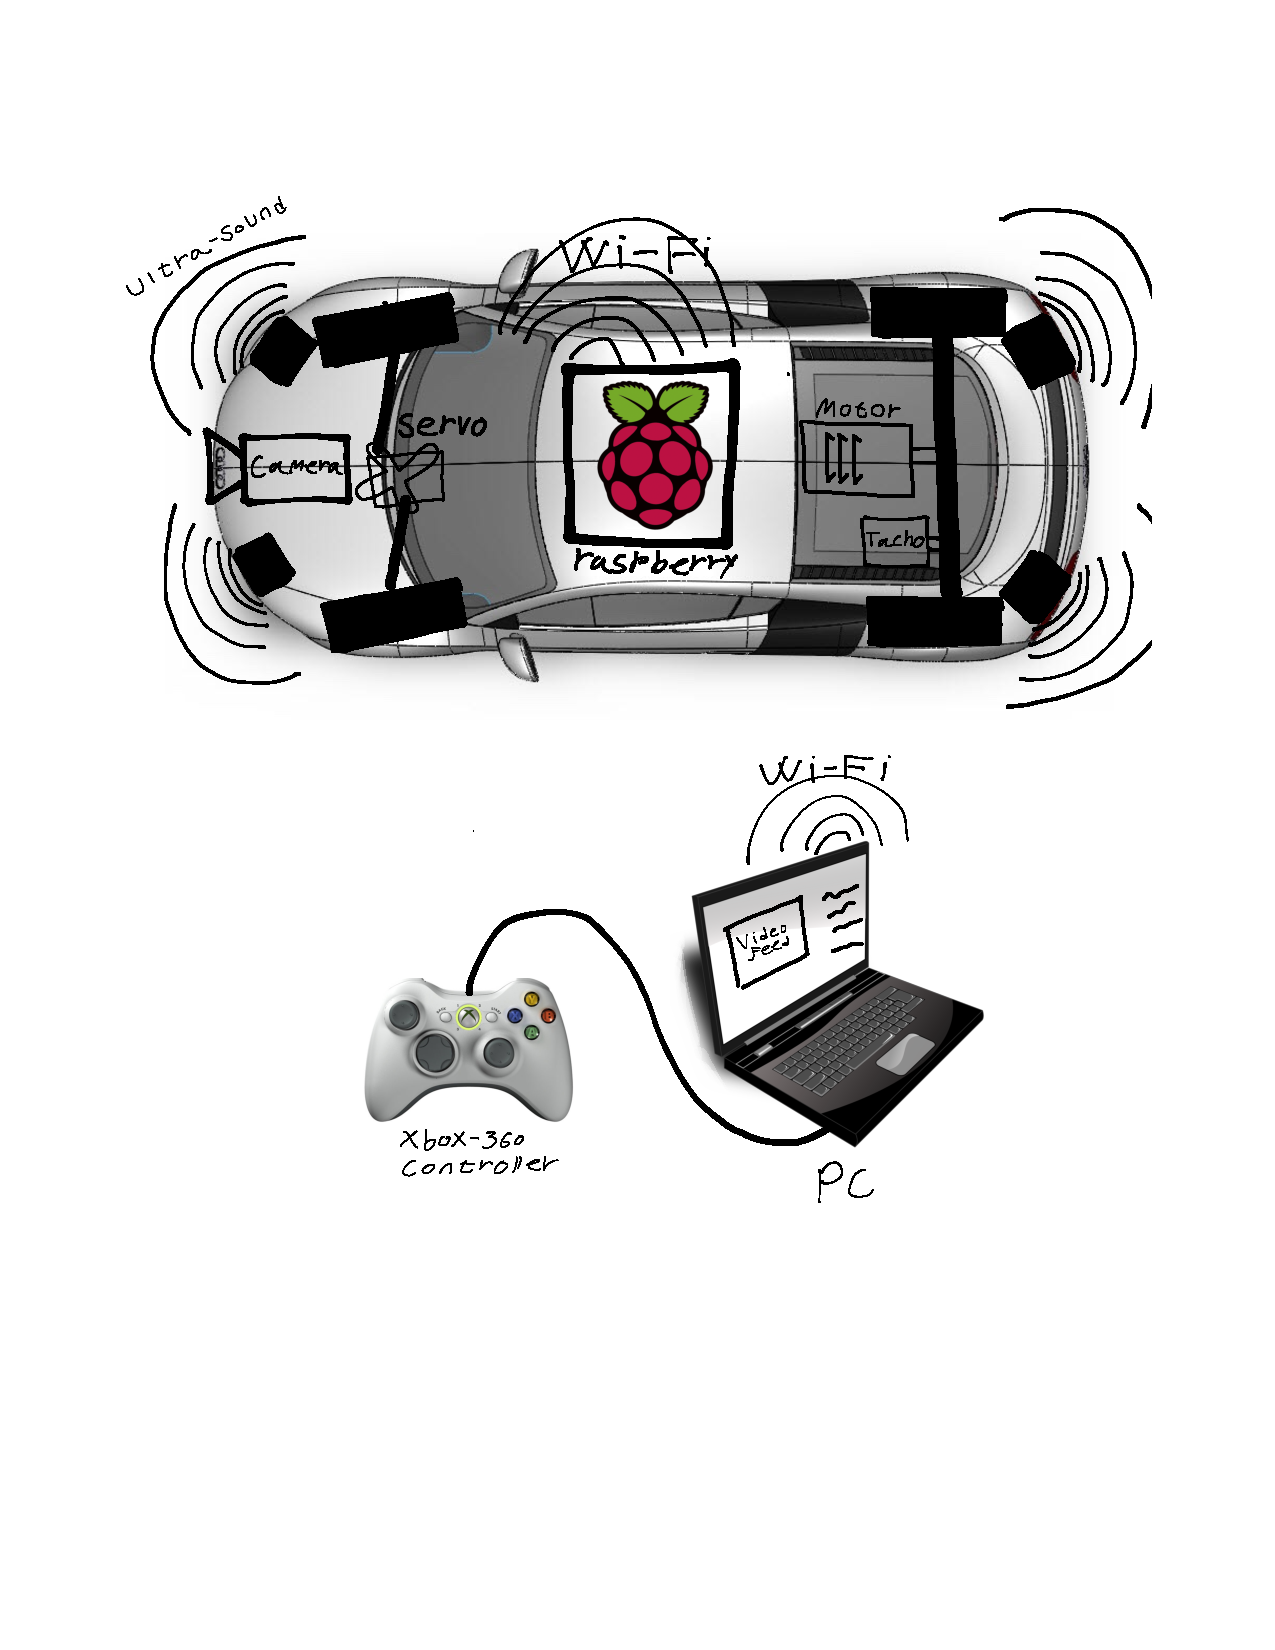
\includegraphics[width=\textwidth - 7.38 cm]{../fig/billeder/rigbillede}
\caption{Rigt billede af samlet system}
\label{fig:rigbillede}
\end{figure} 
AKS systemet er bestående af fire distance sensorer, som er monteret på bilen således de kan detektere forhindringer forud og bagud, samt hvilken side forhindringen er til. På denne måde kan bilen vide om den skal dreje til højre eller venstre for at undgå en kollision. Forhjulene styres med en servomotor som ændre forhjulenes position når brugeren ændre posotionen af venstre styreping på Xbox-360 controlleren. Motoren regulerer bilens hastighed ved hjælp af tacometeret således maksimal acceleration altid opnås når brugeren ændre positionen af knappen \texttt{RT} eller \texttt{LT} på controlleren. Klikker brugeren på \texttt{X} bremses bilen. Tacometeret bruges også til at sende bilens nuværende hastighed til PC'en. På GUI'en modtages data i de lysegrå felter. De mørkegrå felter er knapper som brugeren bruger til at indstille bilens makshastighed, konfigurere IP-adressen til bilen, oprette forbindelse, kalibrere styretøj, tænde eller slukke for AKS samt lukke systemet ned. Se figur \ref{fig:main_menu}. Når brugeren starter GUI'en på PC'en indtaster brugeren bilens IP-adresse ved at klikke på \texttt{''Konfigurer IP''}. Herefter oprettes forbindelsen til bilen ved at brugeren klikker på \texttt{''Opret forbindelse''}. Når GUI'en har oprettet forbindelse til bilen vises der et video-stream og brugeren ser en meddelelsesboks hvori der gives besked om at forbindelsen er oprettet. Brugeren kan nu manøvrere bilen efter sit ønske, eller benytte GUI'ens muligheder om at indtaste en makshastighed, samt tænde eller slukke for AKS systemet. For at brugeren altid kan sikre sig bilen kører lige ud, når venstre styrepind på Xboc-360 controlleren står i midterpositionen, kan brugeren indtaste en kalibreringsværdi som gør at bilen selv tager højde for en eventuelt skævhed i styretøjet.


\begin{figure}[h]
\centering
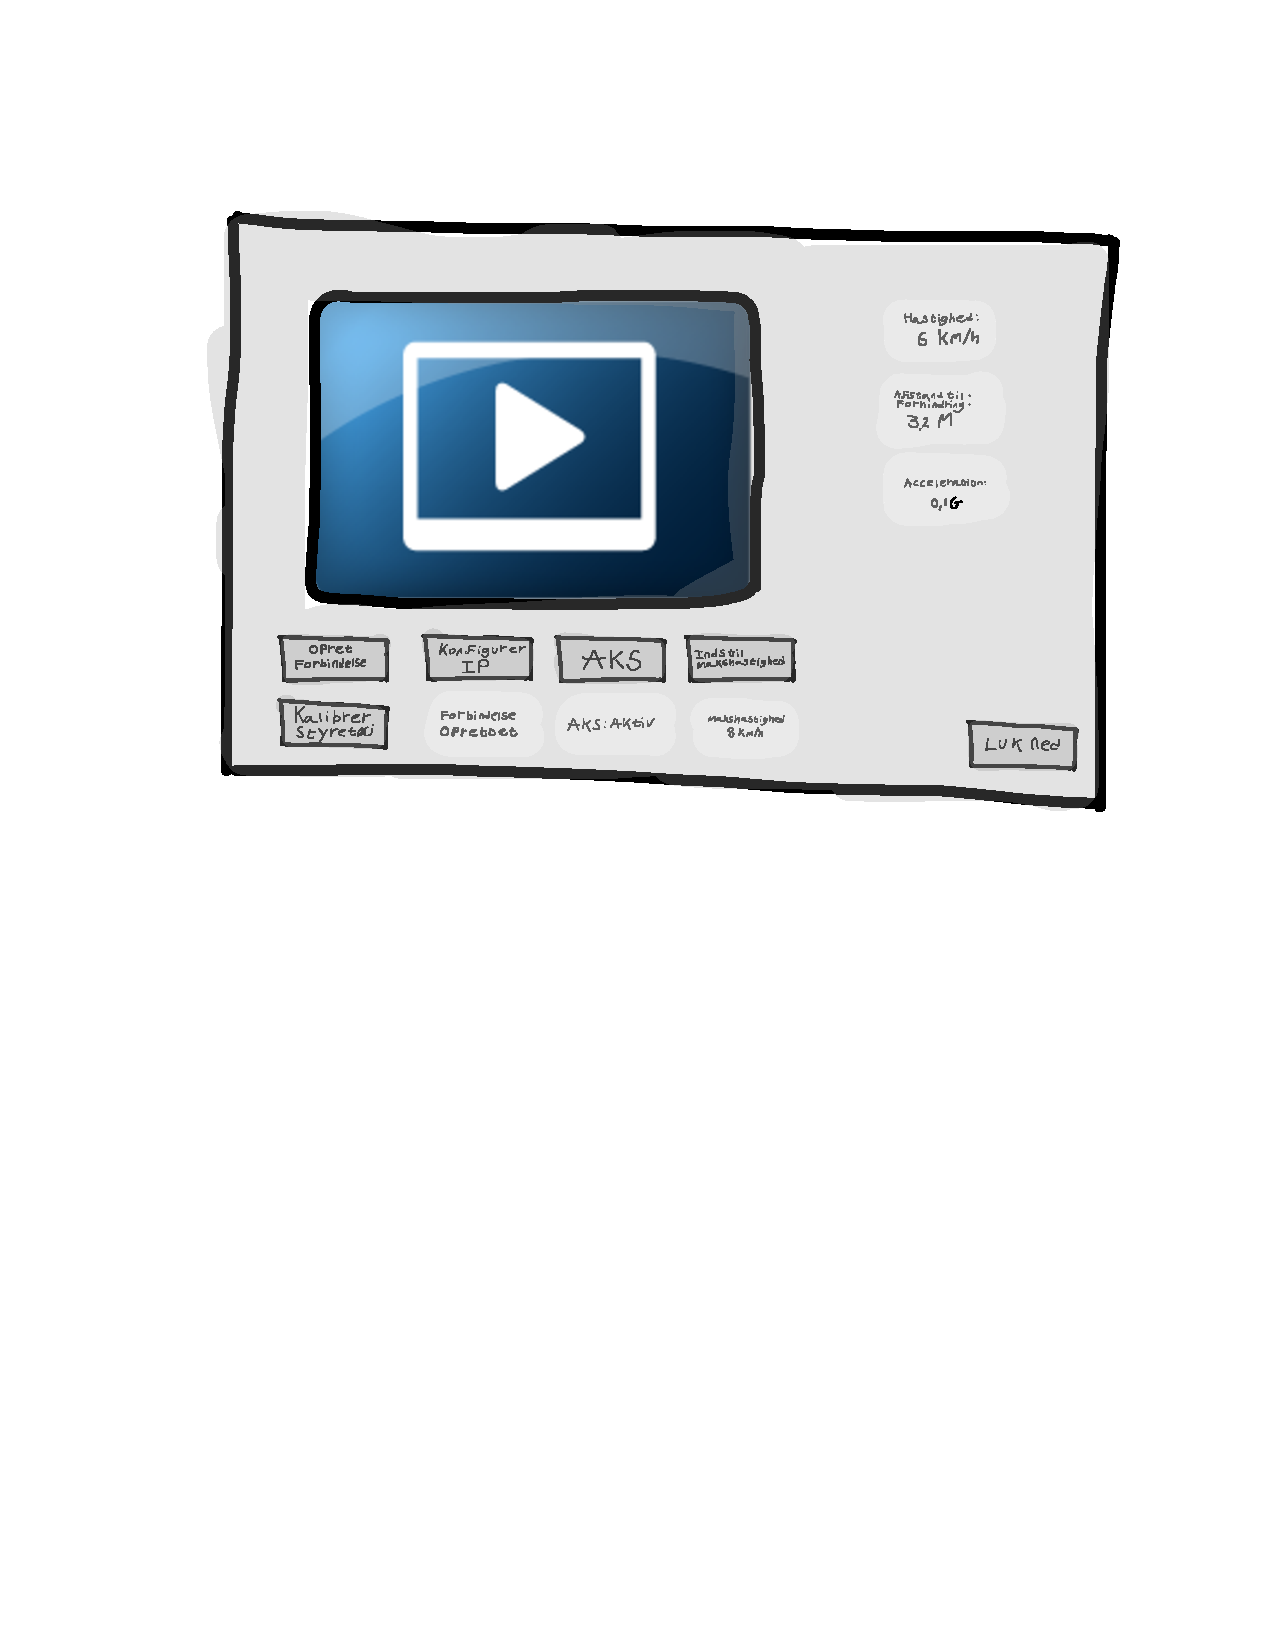
\includegraphics[width=\textwidth*2/3]{../fig/gui/hovedmenu}
\caption{Skitse af hovedmenu}
\label{fig:main_menu}
\end{figure}
